\chapter{Pravděpodobnost v rozhodování a řízení}
\section{Pokusy, jak určit míru nejistoty}
\subsection{Klasická koncepce}
	\begin{itemize}
		\item pojem \textbf{elementárních jevů}
		\item složitý jev se rozkládal na elementární jevy se \textbf{stejnou pravděpodobností výskytu}
		\item pravděpodobnost se určovala jako poměr počtu příznivých jevů ku počtu všech možných jevů
		\item \textbf{nemožným} jevům byla přiřazena 0
		\item \textbf{jistým} jevům byla přiřazena 1
		\item významná vlastnost: čím větší počet pokusů budeme realizovat, tím více se relativní četnost bude blížit pravděpodobnosti $p$.
		\item problém: zpravidla neumíme rozkládat zkoumané jevy na stejně pravděpodobné jevy elementární.
	\end{itemize}
	
\subsection{Relativistická koncepce (statistická pravděpodobnost)}
Statistická pravděpodobnost má větší praktický význam, než klasická koncepce. Spočívá na relativních četnostech výskytu jevů, přičemž množinu všech pozorovaných jevů dělíme na množiny tak, aby každý jev patřil do nějaké skupiny. S rostoucím počtem pozorování se relativní četnosti ustalují kolem určitých čísel. Tato čísla lze považovat za přibližné hodnoty pravděpodobnosti.\br
	
	Změní-li se mechanismus experimentů, nezle používat pravděpodobnost jejich výskytu získané na základě minulých pozorování pro usuzování budoucích výsledků.
	
	\begin{note}{Poznámka}
	Pokud házíme mincí a sledujeme pravděpodobnost, že padne panna, záleží na tom, jestli po celou dobu experimentu používáme stejnou minci. Pokud bychom v půlce experimentu minci ztratili a vzali si jinou, změní se i pravděpodobnost.
	\end{note}
	
	Dalším problémem je, že ne vždy lze na základě pozorování relativní četnosti přisoudit výskytu nějakou pravděpodobnost. Nevýhoda je také, že při stanovení pravděpodobnosti výskytu "řídkých" jevů často vychází nulová relativní četnost i v případě, že jde o jev možný.
	
	\subsection{Subjektivní pravděpodobnost}
	Praxe si vytvořila další koncepci míry nejistoty, a to právě tzv. \textbf{subjektivní pravděpodobnost}. Jedná se o pravděpodobnost, kde expert (někdo, kdo problematice rozumí) určí pravděpodobnost, že nastane daný "řídký" jev. Pravděpodobnost tak závisí právě na zkušenostech tohoto experta. Existují postupy umožňující objektizovat intuitivní rozhodnutí.
	
	\begin{note}{Příklad}
		Musíme se rozhodnout, zda pro výrobu nějakého výrobku zakoupíme licenci za cenu 1 milión Kč, nebo výrobu zajistíme vlastním technickým rozvojem (očekávané náklady 0.5 milionu Kč). Pravděpodobnost úspěšného vývoje je 0.6; pokud bude vývoj neúspěšný, můžeme z hlediska zabezpečení výroby na konci měsíce licenci ještě dokoupit.\br
		
		Musíme porovnat obě varianty:
		\begin{enumerate}[label=\alph*), noitemsep]
			\item nákup licence v ceně 1 mil. Kč
			\item vlastní vývoj, očekávané náklady $0.5 + 1\cdot 0.4 = 0.9$ mil. Kč.
		\end{enumerate}
		
		Z hlediska nákladů je lepší jít cestou vlastního vývoje (optimální rozhodnutí strategie). 
		
		\subsubsection*{Pochybnost o reálnost výpočtu}
		Buď bude vývoj úspěšný - potom budou náklady $0.5$ milionu, nebo bude vývoj neúspěšný, pak budou náklady $0.5+1$ mil. Kč a nikoliv pouze 400 tisíc.\br
		
		Pokud bychom mohli rozhodnutí realizovat 100x, pak by měl výpočet praktický smysl: v 60 případech by stál vývoj 0.5 mil Kč a ve 40 případech by byly náklady ve výši 1.5 mil. Kč. Naše pochybnost vyvěrá  ze skutečnosti, že daný případ je "jedinečný", těžko lze uvažovat o jeho opakovatelnosti, což tuto teorii bortí.\br
	\end{note}
	
	Teprve ve 40 letech v souvislosti s rozpracováním teorie her ukázal von Neumann a Morgenstern smysl, výběru optimální strategie v jedinečných situacích (pokud se v jedinečných situacích zachováme optimálním způsobem, z dlouhodobého hlediska dosáhneme optimální či minimální ceny).\br
	
	Zvolí-li pozorovatel při svém rozhodování v každé jedinečné situaci optimální strategii, zabezpečí si tím dlouhodobě optimální chování. Ke "zhromadnění" jevů, o nichž rozhoduje, dochází v čase "horizontálně" (i když jde pokaždé o jiný jev). Z tohoto přístupu se musí vyloučit tzv. "vitální" případy, jejichž případný neúspěch by mohl ohrozit každou další činnost.
	
	\section{Subjektivní pravděpodobnost}
	Rozklad na elementární jevy ani použití četností není v takových případech možné. Tady přichází tzv. \textbf{subjektivní pravděpodobnost}, což představuje míru nejistoty přiřazená pozorovanému nejistému jevu subjektem rozhodování na základě osobní zkušenosti.
	
	\begin{note}{Příklad}
	Opět zkoumáme vývoj nějakého výrobku nebo racionalizaci nějakého stávajícího výrobku. Vyjdeme z předpokladu, že naše zdroje (materiál, pracovní kapacita, apod) můžeme použít buď na \textbf{vývoj nového výrobku} (technologie) nebo na \textbf{racionalizaci stávajícího výrobku} (technologie).\br
	
	Na základě hrubého rozboru jsme dospěli k závěru, že pokud bude vývoj úspěšný, dojdeme k zisku 500 peněžních jednotek. V případě neúspěchu bude zisk nulový.\br
	
	Zkušenosti subjektu rozhodování využijeme k určení prahu minimálního nutného ziskového přínosu druhé strategie, aby se obě strategie jevily jako ekvivalentní (i s uvážením nejistoty první strategie).
	
	\begin{table}[H]
	\centering
	\def\arraystretch{1.25}
	\begin{tabular}{|c|c|c|}
	\hline
	& $P_0$ (neúspěch) & $P_1$ (úspěch)\\\hline
	Vývoj & 0 & 500\\\hline
	Racionalizace & \multicolumn{2}{|c|}{$K$}\\\hline
	\end{tabular}
	\end{table}		
	
	Symboly $P_0$ a $P_1$ značí pravděpodobnost, kterou subjekt přikládá úspěchu či k neúspěchu. V případě racionalizace předpokládáme zisk $K$ s pravděpodobností 1 (s jistotou).\br
	
	Pro jaké $K$ budeme dávat přednost racionalizaci, případně vývoji:
	\begin{itemize}[noitemsep]
		\item Pro $K=0$ dáváme přednost vývoji
		\item Předpokládáme, že při $K=300$ budeme považovat obě strategie za \textbf{rovnocenné}.
		\item Pro $K < 300$ se tedy budeme rozhodovat pro vývoj a pro $K>300$ se rozhodneme pro racionalizaci.
	\end{itemize}
	
	Předpoklad, že obě strategie budeme považovat za rovnocenné, lze zapsat jako $0\cdot P_0 + 500\cdot P_1=300$, odkud můžeme zjistit, že $P_1 = \frac{300}{500} = 0.6$. Jelikož součet $P_0+P_1=1$, pak $P_0=0.4$.\br
	
	Uvedený postup určení pravděpodobnosti lze objektivizovat tak, že by odhad provedlo nezávisle na sobě několik odborníků schopných posoudit danou situaci a na základě jejich odhadů bychom dostali objektivnější odhad pravděpodobnosti.
	\end{note}
	
	\section{Axiomatická teorie pravděpodobnosti}
	Některé jevy lze jednoznačně předvídat, jiné nikoliv, ale lze pozorovat jisté zákonitosti, pokud jsou opakovány. Pak mluvíme o pravděpodobnostních nebo stochastických zákonitostech.
	
	\begin{itemize}[noitemsep]
		\item Model (přírodních) jevů a uspořádané pozorování jevů nazýváme \textbf{experiment}.
		\item Podmínky experimentu 
		\item Výsledky experimentu, které představují algebru možných výsledků
		\item Složený experiment - výsledky jsou logickou kombinací výsledků dílčích experimentů
		\item Nezávislé experimenty (výsledky jednoho experimentu neovlivní výsledky jiného)
		\item Opakovaný experiment - fundamentální nástroj věděckých disciplín
		\item Princip setrvačnosti přírodních zákonitostí (zákonitosti platí i v budoucím experimentu).
	\end{itemize}
	
	Přiřazování pravděpodobnosti jevů oproti přiřazování nezáporného čísla podmnožinám základní množiny. Přiřazování má vlastnost míry na algebře jevů. To znamená, že teorie pravděpodobnosti je součástí teorie míry na vhodném měřitelném prostoru $(X,\mathscr{U})$. Jev a měřitelná množina jsou tedy synonymy.
	
	\subsection{Pravděpodobnostní prostor}
	Nechť je dána neprázdná množina $\Omega$, která se nazývá \textbf{základním prostorem} a prvky této množiny označené $\omega\in\Omega$ nazýváme výsledky experimentu a nechť je dán soubor $\mathscr{F}$ podmnožin $A$ základního prostoru $\Omega$ a prvky $A$ nazýváme \textbf{pravděpodobnostní jevy} a nechť platí:
	
	\subsubsection*{Axiomy měřitelného prostoru}
		\begin{itemize}[noitemsep]
			\item $\Omega\in\mathscr{F}$
			\item Jestliže $A\in\mathscr{F}$, pak doplněk $A^C\in\mathscr{F}$, kde $A^C$ je doplněk $A$ do množiny $\Omega$
			\item Jestliže $A_1,A_2,\ldots, A_n\in\mathscr{F}, i=1,2,\ldots,n$, pak platí
			\[ \bigcup_{i=1}^\infty A_i\in\mathscr{F} \]
		\end{itemize}
		
		nechť je dále dáno pravděpodobnostní zobrazení $P: \mathscr{F}\to\mathbb{R}$, pro které je dáno
	\subsubsection*{Axiomy pravděpodobnostního zobrazení}
		\begin{itemize}[noitemsep]
			\item $P(A)\geq 0$
			\item $P(\Omega)=1$
		\end{itemize}
		
		Jestliže $A_i\in\mathscr{F}$ a $A_i\cap A_j=\emptyset$ pro $i\neq j$, pak $P(A_1)+P(A_2)+\ldots$\br
		
		Uspořádaná trojice $\{\Omega,\mathscr{F},P\}$ se nazývá \textbf{pravděpodobnostním prostorem}. $\Omega$ představuje základní množinu, jevový prostor, prostor elementárních jevů. $\mathscr{F}$ představuje $\sigma$-algebru podmnožiny množiny $\Omega$ a $P$ pravděpodobnost míry definované na $\mathscr{F}$.
		
		\begin{note}{Motivační příklad}
		\textbf{Podmíněná pravděpodobnost} - střelba na cíl, kde jev $A$ značí zasažení horní poloviny a jev $B$ zasažení pravé poloviny. Pravá horní část je průnikem $A\cup B$.\br
		
		\begin{figure}
			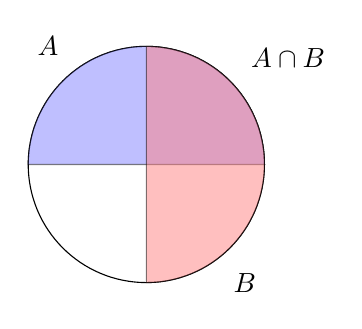
\begin{tikzpicture}
			\draw (0,0) circle [radius = 1.5cm];
			\draw[fill=blue!50, opacity = .5] (1.5,0) arc(0:180:1.5) -- cycle;
			\draw[fill=red!50, opacity=.5] (0,1.5) arc(90:-90:1.5) -- cycle;
			\node (A) at (-1.25, 1.5) {$A$};
			\node (AcB) at (1.8, 1.35) {$A\cap B$};
			\node (B) at (1.25, -1.5) {$B$};
\end{tikzpicture}
		\end{figure}
		\end{note}
	
		Nechť $n_A,n_B, n_{A\cap B}$ a $n_\Omega$ reprezentují počet experimentů, kdy nastal příslušný jev.
		
		\begin{eqnarray*}
			n_A & \simeq & P(A)n_\Omega\\
			n_B & \simeq & P(B)n_\Omega\\
			n_{A\cap B} & \simeq & P(A\cap B)n_\Omega
		\end{eqnarray*}
		
		Dosadíme-li $n_\Omega=\frac{n_B}{P(B)}$, dostaneme
		\[ n_{A\cap B} \simeq \frac{P(A\cap B)}{P(B)}n_B \]
		
		uvažujeme soubor experimentů, kdy jev $B$ nastal $n_B>0$, pak počet experimentů, kdy nastal jev $A$ a zároveň jev $B$ je $n_{A\cap B}$ a tento je úměrný počtu $n_B$.\br
		
		Za těchto podmínek je tedy jev $A$ pravděpodobnostním jevem s pravděpodobností 
		\[ P(A|B) = \frac{P(A\cap B)}{P(B)}, \]
		
		kterou nazveme \textbf{podmíněnou pravděpodobností} jevu $A$ za předpokladu, že nastal jev $B$.
		
		\subsection{Nezávislost jevů}
		Jestliže platí $P(A|B)=P(A)$, pak je jev $A$ nezávislý na jevu $B$. Jestliže jev $A$ nezávisí na jevu $B$, je také jev $B$ nezávislá na jevu $A$.
		
		\begin{note}{Důkaz}
			Víme, že $P(A|B)P(B) = P(B|A)P(A)$. Odtud zjistíme, že $P(A|B)P(B)=P(A)P(B)=P(B|A)P(A)$, z čehož vyplývá, že $P(B|A) = P(B)$.
		\end{note}
		
		\subsection{Zobecnění (nezávislost více jevů)}
		Jevy $A_1,A_2,\ldots$ jsou nezávislé, jestliže pro každou podmnožinu $K_1,K_2,\ldots,K_n$ množiny přirozených čísel platí
		
		\[ P(A_{K_1},A_{K_2},\ldots,A_{K_n}) = P(A_{K_1})\cdot P(A_{K_2})\cdot \ldots\cdot P(A_{K_n}) \]
		
		\textbf{Pozor!} Nezávislost dvou jevů neimplikuje nezávislost skupiny více jevů. Nezávislost skupiny jevů neimplikuje nezávislost vlastních podskupin jevů.